\section{Attempt Level}
\label{sec:attempt}

% Plan (paper_kit/11_paper_outline.md, part 4; about 1.2 pages; claims U5-U11 of 01_thesis_and_claims.md):
% Fig. 2 -- all pairs versus pairs of finished attempts, the baseline "not finished", S under two training schemes,
% S+O; AUROC ceiling and variance shares in two sentences (Figure 3 is not needed); best-of-k in two sentences, no table.
% Sources: paper_kit/06_results_run_level.md; figure: paper_kit/10_figures_tables.md (Figure 2).
\TODO{text of the attempt-level section}

% Caption: paper_kit/10_figures_tables.md, Figure 2, "Подпись (EN)", verbatim.
\begin{figure}[t]
\centering
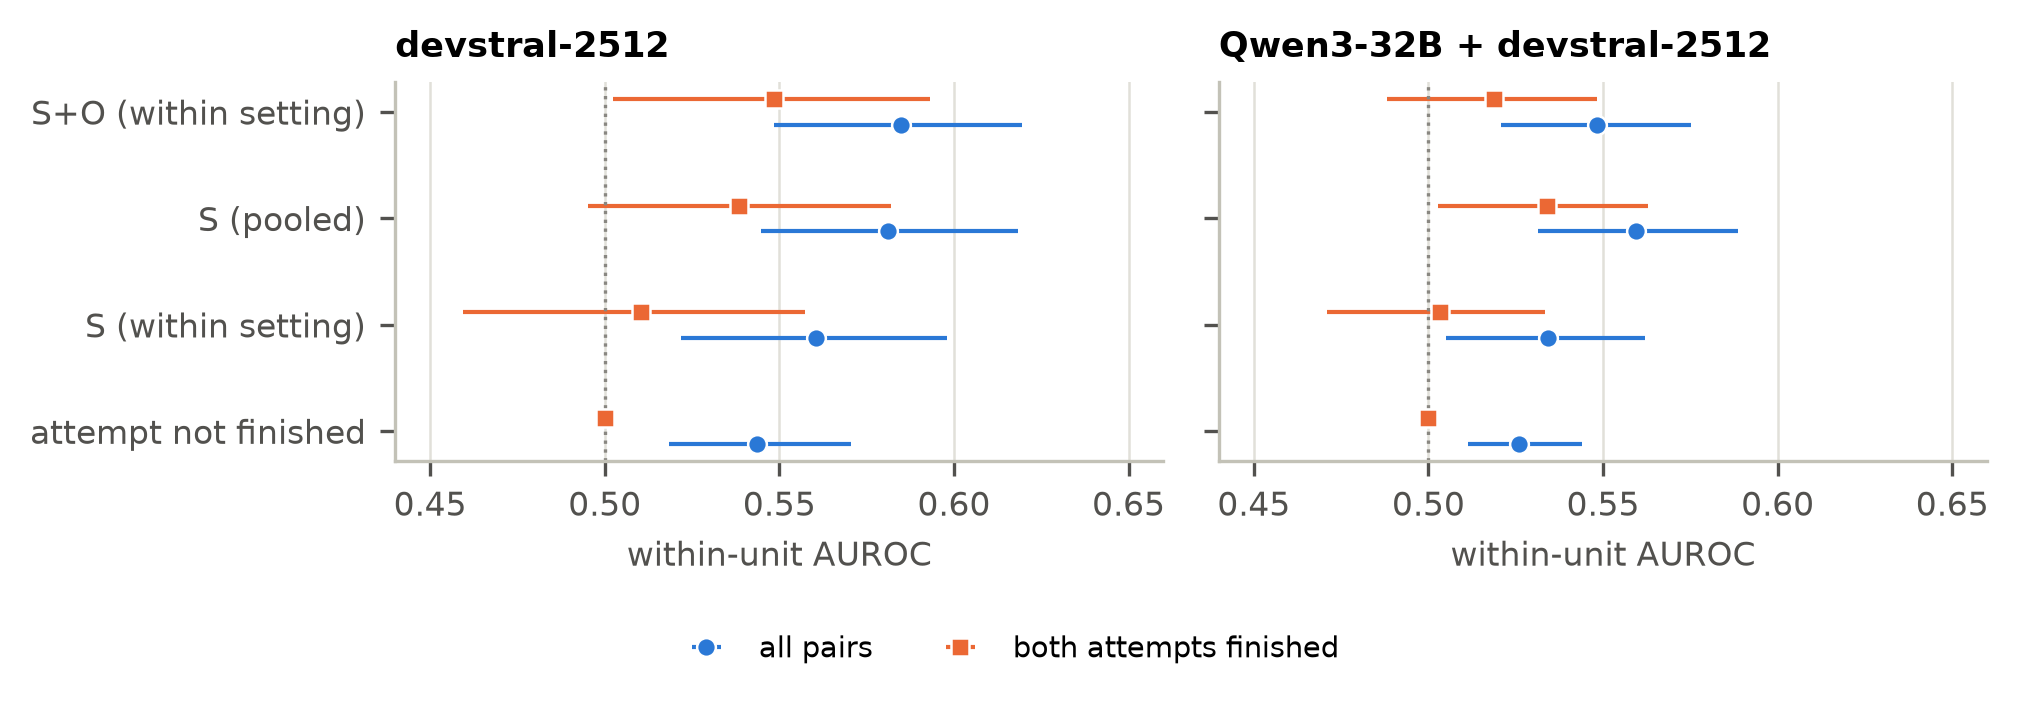
\includegraphics[width=\columnwidth]{fig2_run_level}
\caption{Within-unit AUROC on repeated runs (ASSERT-KTH, two settings). On all pairs the structure model is close to
the single flag `attempt not finished'. Among pairs of finished attempts it is not distinguishable from chance in
either setting (\numsrc{e15k.dev.s2.ff@L120}{0.510 [0.459;\,0.557]} for devstral-2512 with within-setting training);
pooled over both settings it is \numsrc{e15k.both.s1.ff@L128}{0.534 [0.503;\,0.563]} with pooled training and
\numsrc{e15k.both.s2.ff@L130}{0.503 [0.471;\,0.533]} with within-setting training. The agent's own check outcomes
keep a small signal for devstral-2512 (\numsrc{e15k.dev.so2.ff@L123}{0.549 [0.502;\,0.593]} on finished pairs; no
correction for multiple comparisons). Error bars: bootstrap confidence intervals over units.}
\label{fig:run-level}
\end{figure}
